\chapter{Research}
\label{research}

%\section{Introduction to Machine Learning}			
%\section{Artificial Neural Networks}				
%\section{ANNs vs CNNs} 					% disabled for now
%\section{The Perceptron}
%	\subsection{Linearly Separable attribute}		** (img)
%	\subsection{Training Rule}
%	\subsection{Delta Rule and Gradient Descent}
%	\subsection{Derivation of Gradient Descent}
%	\subsection{Gradient Descent Algorithm}
%	\subsection{Stochastic Approximation}
%\section{Multilayer Perceptron Networks}
%	\subsection{Is a perceptron valid for MLP? The Sigmoid Unit}
%	\subsection{Backpropagation Algorithm}
%\section{Face Recognition using CNNs}		% disabled for now
%\section{Voice Recognition}				% disabled for now
%\section{Public Data Sets}
%\section{Python}													

\section{Introduction to Machine Learning}
Machine learning is a term difficult to define, it can be seen from many points of view: it could be Data Mining (applied to databases), Inference (Statistics) or Pattern Recognition (Engineering). One clear thing is that machine learning is a field of artificial intelligence that studies systems that can learn from data. As Kevin P. Murphy said, "The goal of machine learning is to develop methods that can automatically detect patterns in data, and then to use the uncovered patterns to predict future data or other outcomes of interest". 

Within machine learning we can find two different approaches: supervised or unsupervised learning. If you suppose you are providing solution to your kids for each and every situation in their life, it is called they are supervised. But, if your kids take their decisions out of their own understanding, it is called they are unsupervised . Well, something similar happens with machine learning. If you train your model for every input with a corresponding target, then it is supersived learning (you give extra information apart from the data itself) and it will be able to provide target for any new input after sufficient training. Contrary, if you train your model with only a set of inputs it is unsupervised learning and it will be able to find relationships between the different inputs (\cite{sup_unsup_learning}). 

\section{Artificial Neural Networks}
Artificial Neural Networks (ANN) have generated a lot of excitement in Machine Learning research and industry, thanks to many breakthrough results in speech recognition, computer vision and text processing. It is a computational model that is inspired by the way biological neural networks in the human brain process information (\cite{intro_ann}). 

ANN are based in singular units of computation, called neurons, nodes or simplyly units. It receives input from some other nodes, or from an external source and computes an output. Each input has an associated weight ($w$), which is assigned depending of its relative importance to other inputs. The node applies a function $f$ to the weighted sum of its inputs, as we can see in the next figure (\cite{intro_ann}).

\begin{figure}[ht]
	\centering
	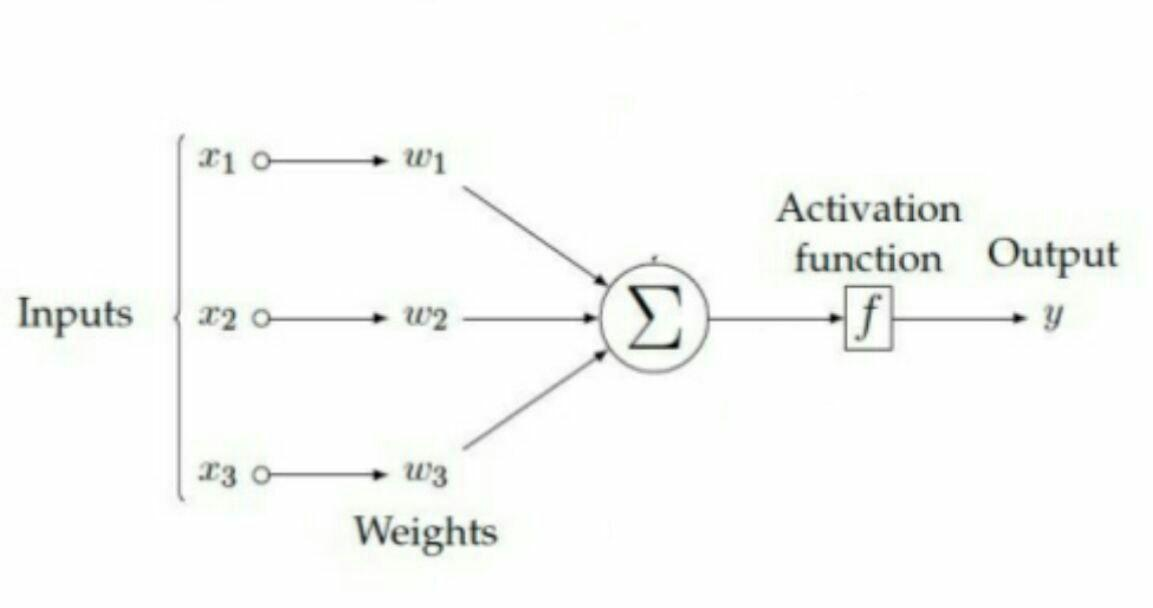
\includegraphics[width=\textwidth]{neuron.jpg}
	\caption{Neuron model}
\end{figure}

These neurons are arranged in layers to construct an ANN. Nodes from adjacent layers have connections between them, so each connection has associated a weight. Because of the position of these nodes and the connections between them we can differentiate three types of nodes: input, hidden and output nodes. 

\begin{figure}[ht]
	\centering
	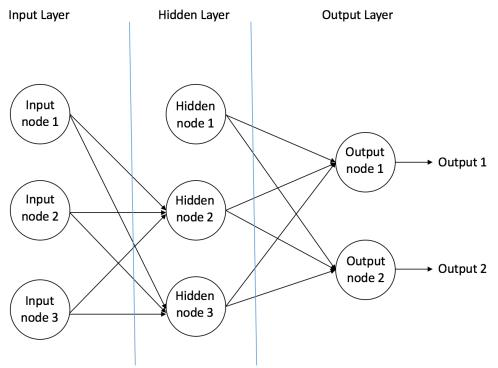
\includegraphics[width=\textwidth]{ann_basic_model.jpg}
	\caption{Basic Artificial Neural Network}
\end{figure}

\begin{itemize}
	\item Input Nodes. Provide information from the outside world without computing anything, they just past the information to the hidden nodes. Together are referred to as the \textit{Input Layer}. 
	\item Hidden Nodes. They have no connection with the outside world (hence the name "hidden"), but they compute the information provided from the previous layer and give the output to the next one. Together are referred to as the \textit{Hidden Layer}. Although these networks must have only one input layer and one output layer, they can have more than one hidden layer (or none). 
	\item Output Nodes. Together are referred to as the \textit{Output Layer} and they are responsible to transfer the computed information to the outside world again.
\end{itemize}

\section{The perceptron}
Within the Artificial Neural Networks (ANN), we can find great variety of units that define the type of ANN involved, but in order to explain how they work, we are going to use a perceptron. This unit has several inputs that are used to perform an operation involving all of them, to finally calculate a single value as a result in a single output.

Each input is composed of a value and a weight, which will indicate the contribution that will contribute to the output of the perceptron. The operation involving all inputs is a linear combination:

\begin{equation}
    \label{linear_combination}
        y=\sum_{i=0}^{n} w_n x_n = w_0 + w_1 x_1 + w_2 x_2 + w_3 x_3 + ...%
\end{equation}

where $x_n$ are the inputs of the perceptron and $w_n$ are the weights ($x_0=1$ is not an input, it's an useful constant to allow us to write the linear operation with a summatory). Finally, the (unique) output of the perceptron depends on the result of the linear operation, being 1 if the result is positive; or -1 in another case. All these data allow us to define the perceptron as follows:

\begin{equation}
    \label{perceptron_rule}
	perceptron(y) =
		\begin{cases}
	     	1 & \text{if $y>0$} \\
	        -1 & \text{otherwise} \\
		\end{cases}
\end{equation}

	\subsection{Linearly Separable attribute}
	This atribute refers to the fact that an hyperplane can separate (or not) the different output values of the perceptron, dividing the space in two sides where there is only one kind of output (1 or -1). To explain it better, we are going to use a percetron with two inputs. With this inputs we can produce a Cartesian map (first input would be X axis; and second input, Y axis). Instead of using a point to represent the input, we use the output symbol (``"+``" or ``"-``"). If we can draw a line (our hyperplane in a 2-dimension space) that divides the map in two sides, so that on each side of the line we can only find one kind of symbol (all positives or all negatives), then we can say that the set of points we have used is linearly separable.  
	
	With a single perceptron there are sets of points that can't be linearly separable. That's why networks of perceptrons with more than one layer are created, whose first layer perceptron's outputs is not the final result, but performs the role as input to another perceptron in the next layer. This way, even the non-linear surfaces can be represented.

	\subsection{Training Rule}
	In order to train perceptrons, we begin assigning random values to the weights and then we apply the perceptron to each training example. If the perceptron misclassifies an example, the training rule will modify the weights according to:

	\begin{equation}
		\label{training_rule}
		w_{i}^{'} \leftarrow w_{i} + \eta (t - o) x_{i}
	\end{equation}

	where $\eta$ is the \textit{learning rate} (constant usually small that determines how much weights vary in each step), $t$ is the target value, $o$ is the actual output that we have obtained from the perceptron and $x_{i}$ is the input value.

	The weights will converge to a value that classify correctly within a finite number of iterations if (and only if) examples are linearly separable and the $\eta$ value used is sufficiently small.
	
	\subsection{Delta Rule and Gradient Descent}
	When the input set is not linearly separable, we need an alternative to the training rule: delta rule. Delta rule uses gradient descent to search for the hypothesis space (set of outputs) that best fit the training example. 

	To explain this we’re going to use a linear unit (not thresholded as the perceptron) which output is calculated by $o = \vec{w} \cdot \vec{x}$. To measure the training error we’re going to use the next formula, where $D$ is the set of examples. It depends only of $\vec{w}$ because we assume that its relation with the examples set $\vec{x}$ will be gone after the training.

	\begin{equation}
		\label{error_function_full_square}
		E(\vec{w}) = \frac{1}{2} \sum_{d \varepsilon D} (t_d-o_d)^2 
	\end{equation}

	If error is defined by this formula, its representation (assuming two inputs) would be a parabolic surface with only one local minimum. The gradient descent will start using a random initial vector and the algorithm will modify its direction step by step. In each step, the algorithm will choose the variation that go the deepest along the error surface. By this way, the process will continue until the local (and global minimum in this case) is reached.

	\begin{figure}[ht]
		\centering
		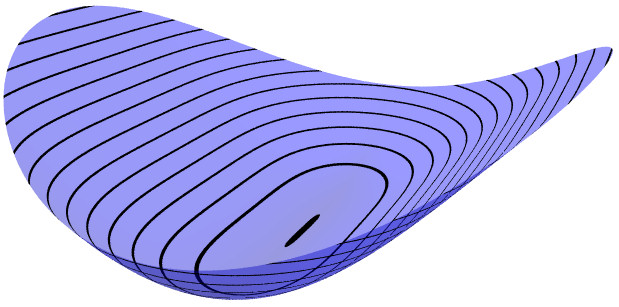
\includegraphics[width=\textwidth-30mm]{parabolic_surface.jpg}
		\caption{Parabolic Surface with one local minimum}
	\end{figure}

	\subsection{Derivation of Gradient Descent}
	To modify the direction of the vector we will derivate the error function ($E(\vec{w})$) respect of $\vec{w}$, form that is called \textit{gradient of E}:

	\begin{equation}
		\label{gradient_of_E}
		\nabla E(\vec{w})= [\frac{\partial{E}}{\partial{w_{0}}}, \frac{\partial{E}}{\partial{w_{1}}}, ..., \frac{\partial{E}}{\partial{w_{n}}}]
	\end{equation}

	This vector specifies the direction that produces the steepest increase in E, so including a negative factor ($-1$) we can calculate the steepest decrease in E. We can represent the training rule with its component form:

	\begin{equation}
		\label{training_rule_component_form}
		w_{i}^{'} \leftarrow w_{i} + \Delta w_{i} \hspace{1.5cm} ; \hspace{1.5cm} \Delta{w_{i}}=-\eta \frac{\partial{E}}{\partial{w_i}}
	\end{equation}

	So the final expression of the gradient descent is:

	\begin{equation}
		\label{gradient_descent_final_expr}
		\Delta w_i = -\eta \frac{\partial{E}}{\partial{w_i}} = \eta \sum_{d \varepsilon D} (t_d - o_d) x_{id}
	\end{equation}


	\subsection{Gradient Descent Algorithm}
	A brief version of the algorithm would be as follows:

	\begin{enumerate}

		\item Pick an initial random weight vector.
		\item Apply the linear unit to all training examples and then compute $\Delta w_i$  using the gradient descent formula.
		\item Update each weight adding $\Delta w_i$.
		\item If the algorithm hasn’t reached the local minimum, repeat from step 2.
	
	\end{enumerate}

	\subsection{Stochastic Approximation}
	Instead of using all the examples to update the weight each step (which could imply a lot of work) there is another option: incremental/stochastic gradient descent. This way we will approximate the gradient descent updating the weights with each training example:

	\begin{equation}
		\label{delta_rule}
		\Delta w_{i}= \eta (t - o) x_{i}
	\end{equation}

	So the error function must be changed to:

	\begin{equation}
		\label{error_function_stoc_square}
		E(\vec{w}) = \frac{1}{2} (t_d-o_d)^2 
	\end{equation}

\section{Multilayer Perceptron Networks}
A single perceptron can only express linear decision surfaces, so it is very limited for real life situations. In contrast, a multilayer network learned by the backpropagation algorithm can express a rich variety of non-linear decision surfaces, which are more suitable for that kind of problems.

	\subsection{Is a perceptron valid for MLP? The Sigmoid Unit}
	A perceptron unit is perfectly valid for a MLP, but its discontinuous threshold output make it not suitable at all for gradient descent. Also, as a linear unit, multiple layers of cascaded units will only produce linear functions. Then, another option is required: a \textbf{sigmoid threshold unit}. This unit works pretty similar to the perceptron, but has another function at the output to perform the threshold, which is called logistic or sigmoid function ($\sigma(y)$).

		\begin{equation}
			\label{sigmoid_function}
			\sigma(y) = \frac{1}{1+e^{-y}}
		\end{equation}

	This function increases monotonically and continuously with its input and is able to map a large input domain to a small range (0, 1) of outputs, reason because is usually called \textit{squashing function}. Finally, being easy derivable make it a really good choice for our task. 


	\subsection{Backpropagation Algorithm}
	The Backpropagation Algorithm learns the weights for a multilayer  network, given a network with a fixed set of units and interconnections. It uses gradient descent to minimize the squared error between the output and its target values of the network:

		\begin{equation}
			\label{squared_error_function_network}
			E(\vec{w}) = \frac{1}{2} \sum_{d \varepsilon D} \sum_{k \varepsilon outputs} (t_{kd}-o_{kd})^2 
		\end{equation}

	As we have changed the error function definition, the error surface will have more than one local minima (not as before with a single perceptron). This means that gradient descent may fail in order to find the global minima and only reach a local minima instead. Anyway, it has been proved to produce excellent results even with this problem.

	The stochastic version of the Backpropagation Algorithm, applied for each training example, would be:

		\begin{enumerate}

			\item Input the values in the network and obtain the output values computing every unit of the network.
			\item For each output unit ($k$), calculate its error term $\delta_k$, which is the usual $(t-o)$ multipied to the derivate of the sigmoid function:
				\begin{equation}
					\label{backpropagation_output_error}
					\delta_k \leftarrow o_k (1 - o_k)(t_k - o_k)
				\end{equation}				

			\item For each hidden unit ($h$), calculate its error term $\delta_h$. This is similar to the output formula, but as we don't have a target value for a hidden unit, we must calculate it summing up the errors of the downstream units weigthing each error by the weight of the connection that links them. 
				\begin{equation}
					\label{backpropagation_hidden_error}
					\delta_h \leftarrow o_h (1 - o_h) \sum_{l \varepsilon downstream} (w_{hl} \delta_i)
				\end{equation}

			\item Update each network weight:
				\begin{equation}
					\label{backpropagation_weight_update}
					w^{'}_{ji} \leftarrow w_{ji} + \Delta w_{ji} \hspace{1.5cm} ; \hspace{1.5cm} \Delta w_{ji} = \eta \delta_j x_{ji}
				\end{equation}

		\end{enumerate} 

%\section{Face Recognition using CNNs}

%\section{Voice Recognition}	% disabled for now

\section{Public Data Sets} 
Face recognition is nothing but another kind of machine learning and as such, it needs to be feeded with data, face images in this case. The problem is that we need a high amount of them, in addition to that each face image has to be different (or the model would only work well with the data we worked with, and not any face, which is our purpose). As we cannot generate this dataset by ourselves, we must look for a public dataset with enough and different face images:

\begin{itemize}
	\item CASIA Webface Database. It is the second largest database of faces (first is private and belongs to Facebook), with more than 10,000 subjects and almost 500,000 images. In order to use it an agreement needs to be signed so the database will only be used for non-comercial, research or educational purposes. We finally discarded it because its size, which would be more suitable for a big project with a research group (\cite{casia_db}). 
	\item WIDER FACE. This database counts with more than 32,000 images and can be freely accessed by a Google or Baidu Drive. It has the advantage that its images are already labelled and the faces in them are marked. However, many of the images have more than one face on them (they say they count with almost 400,000 faces in the dataset) and we need them to have only one person (\cite{widerf_db}).
	\item Labelled Faces in the Wild (LFW). This database only counts with more than 13,000 images that only have one person in them, which is perfect for the scope of this project. It can be explored online and has been recently updated, solving some erratum. Finally, it also has the option to download the images aligned with funneling or commercial software, reducing the work to do on the dataset. Because of all these reasons, it is the dataset that is going to be used for the project (\cite{lfw_db}).
\end{itemize}

\section{Python}
In the Introduction of this project we already have enumerated some of the features of this language, but there is much more. First, it is a high-level language designed to be easily readable. One interesting example of this is the lack of brackets ("{}"), which is the usual way to delimit control flow blocks in other languages. Instead, Python uses indentation, so to indicate a line is inside a function or an \textit{if} block, we just have to indent it one level more. We can see it clearly in the next comparative.

\noindent\begin{minipage}[t]{.45\textwidth}
\begin{lstlisting}[caption=C code,frame=tlrb, language=C]{Name}
void foo(int x)
{
    if (x == 0) {
        bar();
    } else {
        foo2(x + 3);
    }
}
\end{lstlisting}
\end{minipage}\hfill
\begin{minipage}[t]{.45\textwidth}
\begin{lstlisting}[caption=Python code,frame=tlrb, language=Python]{Name}
def foo(x):
    if x == 0:
        bar()
    else:
        foo2(x + 3)
\end{lstlisting}
\end{minipage}

Second, Python is interactive. When we install Python in our computer we can launch it in the terminal and a prompt will show up, allowing us to interact with the interpreter directly to write our programs. Directly related with this feature is that Python is interpreted. This means that it does not need to be compiled before executing (what happens to languages like C, C++ or Lisp), as it is processed by at runtime by the interpreter (\cite{python_overview}). 

And finally, Python is easy to learn. It has fewer keywords than other languages, its strucure is much simpler and the syntax is easily readable with a certain level of English. It is because all of this why it has become very popular in recent years, being used from to start learning programming to advanced investigation projects.
